\documentclass[a4paper,11pt]{report}

\usepackage{amsmath,amsfonts,amssymb}
\usepackage{graphics}
\usepackage{graphicx}
\usepackage{booktabs}
\usepackage{tabularx}
\usepackage{array}
\usepackage{icomma}
\usepackage{tikz, ifthen}
\usetikzlibrary{arrows,shapes,backgrounds,patterns,decorations.pathreplacing,decorations.pathmorphing}

% <Temporary FHSST definitions>
\def\Definition#1#2{\paragraph{Definition:} #1 --- #2}

\def\Identity#1#2{\paragraph{Identity:} #1 --- #2}

\newenvironment{wex}[3]%
{\rule{\linewidth}{0.5mm}
\textbf{Worked example:} #1

\textbf{Question:} #2

\textbf{Solution:} #3}%
{\rule{\linewidth}{0.5mm}}

\newcommand{\westep}[1]{\paragraph{Step:} #1}

\newenvironment{example}%
{\rule{\linewidth}{0.5mm}
\textbf{Example:} \\}%
{\rule{\linewidth}{0.5mm}}

\newenvironment{exercises}[1]%
{\rule{\linewidth}{0.5mm}
\textbf{Exercises:} #1\\}%
{\rule{\linewidth}{0.5mm}}

\newenvironment{eocexercises}[1]%
{\section{End of chapter exercises: #1}}%
{}
% </Temporary FHSST definitions>

% <Temporary spacing changes>
\setlength\parindent{0pt}
\setlength\parskip{0.5\baselineskip}
\setlength\textwidth{15cm}
\setlength\textheight{23cm}
\setlength\oddsidemargin{0.5cm}
\setlength\topmargin{0cm}
% </Temporary spacing changes>

\begin{document}
\chapter{Statistics}

\section{Introduction}

When running an experiment or conducting a survey we can potentially
end up with many hundreds, thousands or even millions of values in the
resulting data set. Too many data can be overwhelming and we need to
reduce them or represent them in a way that is easier to understand
and communicate.

Statistics is about summarising data. The methods of statistics allow
us to represent the essential information in a data set while
disregarding the unimportant information. We have to be careful to
make sure that we do not accidentally throw away some of the important
aspects of a data set.

%The figure below shows one example of how we can reduce the complexity
%of a data set while still retaining the important information.

%FIGURE: Side-by-side images of two datasets drawn from the same $2$-d
%normal distribution. $N = 50$. Even though the individual data are
%different, the statistics (central tendency and dispersion) are very
%similar. The statistics capture the interesting aspects of the data.
%\begin{center}
%  \begin{tikzpicture}
%  \end{tikzpicture}
%\end{center}

By applying statistics properly we can highlight the important aspects
of data and make the data easier to interpret. By applying statistics
poorly or dishonestly we can also hide important information and let
people draw the wrong conclusions.

In this chapter we will look at a few numerical and graphical ways in
which data sets can be represented, to make them easier to interpret.

\section{Collecting data}
\Definition{Data}{Data refers to the pieces of information that have
  been observed and recorded, from an experiment or a survey. Note
  that the word {\em data} is the plural of the word {\em datum}, and
  therefore one should say, ``the data are'' and not ``the data is''.}

We distinguish between two main types of data: quantitative and
qualitative.

\Definition{Quantitative data}{Quantitative data are data that can be
  written as numbers.}

Quantitative data can be discrete or continuous. Discrete quantitative
data can be represented by integers and usually occur when we count
things, for example, the number of learners in a class, the number of
molecules in a chemical solution, or the number of SMS messages sent
in one day.

Continuous quantitative data can be represented by real numbers, for
example, the height or mass of a person, the distance travelled by a
car, or the duration of a phone call.

\Definition{Qualitative data}{Qualitative data are data that cannot be
  written as numbers, for example, when you collect responses from
  people about how they feel or what their favourite colour is.}

Two common types of qualitative data are categorical and anecdotal
data. Categorical data can come from one of a limited number of
possibilities, for example, your favourite cool drink, the colour of
your cell phone, or the language that you learned to speak at home.

Anecdotal data take the form of an interview or a story, for example,
when you ask someone what their personal experience was when using a
product, or what they think of someone else's behaviour.

Categorical qualitative data are sometimes turned into quantitative
data by counting the number of times that each category appears.

\begin{example}
  In a class with $30$ learners, we ask everyone what the colour of
  their cellphone is and get the following responses.

  \begin{center}
    \begin{tabular}{cccccccccc}
      \toprule
      black & black & black & white & purple & red & red & black & black & black \\
      white & white & black & black & black & black & purple & black & black & white \\
      purple & black & red & red & white & black & orange & orange & black & white \\
      \bottomrule
    \end{tabular}
  \end{center}

  This is a categorical qualitative data set since each of the
  responses comes from one of a small number of possible colours.

  We can represent exactly the same data in a different way, by
  counting how many times each colour appears.

  \begin{center}
    \begin{tabular}{cc}
      \toprule
      colour & count \\
      \midrule
      black & 15 \\
      white & 6 \\
      red & 4 \\
      purple & 3 \\
      orange & 2\\
      \bottomrule
    \end{tabular}
  \end{center}

  This is a discrete quantitative data set since each count is an
  integer.

\end{example}

\begin{wex}{Qualitative and quantitative data}{
    Andrew is interested in becoming an airtime reseller to his
    classmates. He would like to know how much business he can expect
    from them. He asked each of his $20$ classmates how many SMS
    messages they sent during the previous day. The results were:

    \begin{center}
      \begin{tabular}{rrrrrrrrrr}
        \toprule
        $20$ & $ 3$ & $ 0$ & $14$ & $30$ & $9$ & $11$ & $13$ & $13$ & $15$ \\
         $9$ & $13$ & $16$ & $12$ & $13$ & $7$ & $17$ & $14$ & $ 9$ & $13$ \\
        \bottomrule
      \end{tabular}
    \end{center}

    Is this data set qualitative or quantitative? Explain your answer.
}{
  The number of SMS messages is a count, which means that it is
  quantitative and discrete.

}
\end{wex}

\begin{wex}{Qualitative and quantitative data}{
    Thembisile would like to know who the most popular cellular
    provider is among learners in his school. This time Thembisile
    randomly selects $20$ learners from the entire school and asks them
    which cellular provider they currently use. The $20$ results were:

    \begin{center}
      \begin{tabular}{p{0.17\textwidth}p{0.17\textwidth}p{0.17\textwidth}p{0.17\textwidth}p{0.17\textwidth}}
        \toprule
        Cell C & Vodacom & Vodacom & MTN & Vodacom \\
        MTN & MTN & Virgin Mobile & Cell C & 8-ta \\
        Vodacom & MTN & Vodacom & Vodacom & MTN \\
        Vodacom & Vodacom & Vodacom & Virgin Mobile & MTN \\
        \bottomrule
      \end{tabular}
    \end{center}

    Is this data set qualitative or quantitative? Explain your answer.
}{
  Since each response is not a number, but one of a small number of
  possibilities, these are categorical qualitative data.

}
\end{wex}

\section{Measures of central tendency}

\subsection{Mean}
\Definition{Mean}{The mean is defined as the sum of a set of values,
  divided by the number of values in the sum.  The notation for the
  mean of a set of values is a horizontal bar over the variable used
  to represent the set. The formula for the mean of a data set $\{x_1,
  x_2, \ldots, x_n\}$ is
  \begin{align}
    \overline{x} &= \frac{1}{n}\sum_{i=1}^n x_i \\
                 &= \frac{x_1 + x_2 + \cdots + x_n}{n}
  \end{align}
}

The mean is sometimes also called the average or the arithmetic mean.

\begin{wex}{Calculating the mean}{
    What is the mean of the data set $\{10;\ 20;\ 30;\ 40;\ 50\}$?
}{
  \westep{Compute the sum of the data.}
  \begin{equation}
    10 + 20 + 30 + 40 + 50 = 150
  \end{equation}

  \westep{Divide by the number of values in the data set to get the mean.}

  Since there are $5$ values in the data set, the mean is
  \begin{equation}
    \frac{150}{5} = 30
  \end{equation}
}
\end{wex}

\subsection{Median}
\Definition{Median}{
  The median of a data set is the value in the central position,
  when the data set has been arranged from the lowest to the highest
  value. Exactly half of the values from the data set are less than
  the median and the other half are greater than the median.}

To calculate the median of a quantitative data set, first sort the
data from the smallest to the largest value and then find the value in
the middle. If there are an odd number of data, the median will be
equal to one of the values in the data set. If there are an even
number of data, the median will lie halfway between two values in
the data set.

\begin{wex}{Median for an odd number of values}{
  What is the median of $\{10;\ 14;\ 86;\ 2;\ 68;\ 99;\ 1\}$?
}{
  \westep{Sort the values.}

  The values in the data set, from the smallest to the largest, are
  \begin{equation}
    1;\ 2;\ 10;\ 14;\ 68;\ 86;\ 99
  \end{equation}

  \westep{Find the number in the middle.}

  There are $7$ values in the data set. Since there are an odd number
  of values, the median will be equal to the value in the middle,
  namely, at the $4$th position. The value in the $4$th position is
  $14$ and therefore the median of the data set is $14$.

}
\end{wex}

\begin{wex}{Median for an even number of values}{
  What is the median of $\{11;\ 10;\ 14;\ 86;\ 2;\ 68;\ 99;\ 1\}$?
}{
  \westep{Sort the values.}

  The values in the data set, from the smallest to the largest, are
  \begin{equation}
    1;\ 2;\ 10;\ 11;\ 14;\ 68;\ 86;\ 99
  \end{equation}

  \westep{Find the number in the middle.}

  There are $8$ values in the data set. Since there are an even number
  of values, the median will be halfway between the two values in the
  middle, namely, at the $4$th and $5$th positions. The value in the
  $4$th position is $11$ and the value in the $5$th position is
  $14$. The median lies halfway between these two values and is
  therefore
  \begin{equation}
    \frac{11+14}{2} = 12,5
  \end{equation}
}
\end{wex}

\subsection{Mode}
\Definition{Mode}{
  The mode of a data set is the value that occurs most often in the
  set. The mode can also be described as the most frequent or most
  common value in the data set.}

To calculate the mode, we simply count the number of times that each
value appears in the data set and then find the value that appears
most often.

A data set can have more than one mode if there is more than one value
with the highest count. For example, both $2$ and $3$ are modes in the
data set $\{1;\ 2;\ 2;\ 3;\ 3\}$. If all points in a data set occur
with equal frequency, it is equally accurate to describe the data set
as having many modes or no mode.

\begin{wex}{Find the mode}{
    Find the mode of the data set
    \begin{equation}
      \{2;\ 2;\ 3;\ 4;\ 4;\ 4;\ 6;\ 6;\ 7;\ 8;\ 8;\ 10;\ 10\}
    \end{equation}
}{
  \westep{Count the number of times that each value appears in the data
    set.}

  \begin{center}
    \begin{tabular}{cc}
      \toprule
      value & count \\
      \midrule
      $2$ & $2$ \\
      $3$ & $1$ \\
      $4$ & $3$ \\
      $6$ & $2$ \\
      $7$ & $1$ \\
      $8$ & $2$ \\
      $10$ & $2$ \\
      \bottomrule
    \end{tabular}
  \end{center}

  \westep{Find the value that appears most often.}

  From the table above we can see that $4$ is the only value that
  appears $3$ times, and all the other values appear less
  often. Therefore the mode of the data set is $4$.

}
\end{wex}

One problem with using the mode as a measure of centreal tendency is
that we can usually not compute the mode of a continuous data
set. Since continuous values can lie anywhere on the real line, any
particular value will almost never repeat. This means that the
frequency of each value in the data set will be $1$ and that there will
be no mode. We will look at one way of adressing this problem in
Section \ref{sec:statistics_grouping_data} on grouping data.

\begin{wex}{Comparison of measures of central tendency}{
    There are regulations in South Africa related to bread production
    to protect consumers. By law, if a loaf of bread is not labelled,
    it must weigh $800$ g, with the leeway of $5$ percent under or $10$
    percent over.  Vishnu is interested in how a well-known, national
    retailer measures up to this standard. He visited his local branch
    of the supplier and recorded the masses of $10$ different loaves
    of bread for one week. Here are the results:

    \begin{center}
      \begin{tabular}{ccccccc}
        \toprule
        Monday & Tuesday & Wednesday & Thursday & Friday & Saturday & Sunday \\
        \midrule
        $802,4$ & $787,8$ & $815,7$ & $807,4$ & $801,5$ & $786,6$ & $799,0$ \\
        $796,8$ & $798,9$ & $809,7$ & $798,7$ & $818,3$ & $789,1$ & $806,0$ \\
        $802,5$ & $793,6$ & $785,4$ & $809,3$ & $787,7$ & $801,5$ & $799,4$ \\
        $819,6$ & $812,6$ & $809,1$ & $791,1$ & $805,3$ & $817,8$ & $801,0$ \\
        $801,2$ & $795,9$ & $795,2$ & $820,4$ & $806,6$ & $819,5$ & $796,7$ \\
        $789,0$ & $796,3$ & $787,9$ & $799,8$ & $789,5$ & $802,1$ & $802,2$ \\
        $789,0$ & $797,7$ & $776,7$ & $790,7$ & $803,2$ & $801,2$ & $807,3$ \\
        $808,8$ & $780,4$ & $812,6$ & $801,8$ & $784,7$ & $792,2$ & $809,8$ \\
        $802,4$ & $790,8$ & $792,4$ & $789,2$ & $815,6$ & $799,4$ & $791,2$ \\
        $796,2$ & $817,6$ & $799,1$ & $826,0$ & $807,9$ & $806,7$ & $780,2$ \\
        \bottomrule
      \end{tabular}
    \end{center}

    \begin{enumerate}
    \item Is this data set qualitative or quantitative? Explain your
      answer.
    \item Compute the mean, median and mode of the mass of a loaf of bread
      for each day of the week. Give your answer to one decimal place.
    \item Based on the data, do you think that this supplier is
      providing bread within the South African guidelines?
    \end{enumerate}
}{

  \westep{Qualitative or quantitative?}

  Since each mass can be represented by a number, the data
  set is quantitative. Furthermore, since a mass can be any real
  number, the data are continuous.

  \westep{Compute the mean.}

  In each column (for each day of the week), we add up the
  measurements and divide by the number of measurements, $10$.

  For Monday, the sum of the measured values is $8007,9$ and so the
  mean for Monday is
  \begin{equation}
    \frac{8007,9}{10} = 800,8\textrm{ g}
  \end{equation}

  In the same way, we can compute the mean for each day of the
  week. See the table below for the results.

  \westep{Compute the median.}

  In each column we sort the numbers from lowest to highest and find
  the value in the middle. Since there are an even number of
  measuremnts ($10$), the median is halfway between the two numbers in
  the middle.

  For Monday, the sorted list of numbers is
  \begin{equation}
    789,0;\ 789,0;\ 796,2;\ 796,7;\ 801,2;\ 802,3;\ 802,3;\ 802,5;\ 808,7;\ 819,6
  \end{equation}
  The two numbers in the middle are $801,2$ and $802,3$ and so the
  median is
  \begin{equation}
    \frac{801,2 + 802,3}{2} = 801,8
  \end{equation}

  In the same way, we can compute the median for each day of the
  week. Here is a table with all the means and medians.

  \begin{center}
    \begin{tabular}{lcc}
      \toprule
      \multicolumn{1}{c}{day} & mean & median \\
      \midrule
      Monday & $800,8$ g & $801,8$ g \\
      Tuesday & $797,2$ g & $796.1$ g \\
      Wednesday & $798,4$ g & $797,2$ g \\
      Thursday & $803,4$ g & $800,8$ g \\
      Friday & $802,0$ g & $804,3$ g \\
      Saturday & $801,6$ g & $801,4$ g \\
      Sunday & $799,3$ g & $800,2$ g \\
      \bottomrule
    \end{tabular}
  \end{center}

  From the above calculations we can see that the means and medians
  are close to one another, but not quite equal. In the next worked
  example we will see that the mean and median are not necessarily
  close to each other.

  \westep{Compute the mode.}

  Since the data are continuous we cannot compute the mode. In the next
  section we will see how we can group data in order to make it possible
  to compute an approximation for the mode.

  \westep{Conclusion: Is the supplier reliable?}

  From the question the requirements are that the mass of a loaf of
  bread be between $800$ g minus $5$\%, which is $760$ g, and plus
  $10$\%, which is $880$ g. Since every one of the measurements made
  by Vishnu lies within this range and since the means and medians are
  all close to $800$ g, we can conclude that the supplier is reliable.

}
\end{wex}

\Definition{Outlier}{An outlier is a value in the data set that is not
  typical of the rest of the set. It is usually a value that is much
  greater or much less than all the other values in the data set.}

\begin{wex}{Effect of outliers on mean and median}{
    The heights of $10$ learners are measured in centimetres to obtain
    the following dataset:
    \begin{equation}
      \{150;\ 172;\ 153;\ 156;\ 146;\ 157;\ 157;\ 143;\ 168;\ 157\}
    \end{equation}
    Afterwards, we add one more learner to the group, who is
    exceptionally tall: $181$ cm.

    Compare the mean and median of the heights of the learners before
    and after the $11$th learner was added.
}{
  \westep{Compute the mean with the first $10$ learners.}

  \begin{equation}
    \frac{150 + 172 + 153 + 156 + 146 + 157 + 157 + 143 + 168 + 157}{10}
    = 155,9\textrm{ cm}
  \end{equation}

  \westep{Compute the mean with all $11$ learners.}

  \begin{equation}
    \frac{150 + 172 + 153 + 156 + 146 + 157 + 157 + 143 + 168 + 157 + 181}{11}
    = 158,2\textrm{ cm}
  \end{equation}

  From this we see that the average height changes by
  $158,2 - 155,9 = 2,3\textrm{ cm}$ when we introduce
  the outlier value (the tall person) to the data set.

  \westep{Compute the median with the first $10$ learners.}

  To find the median, we need to sort the data set:
  \begin{equation}
    \{143;\ 146;\ 150;\ 153;\ 156;\ 157;\ 157;\ 157;\ 168;\ 172\}
  \end{equation}
  Since there are an even number of values, namely $10$, the median
  lies halfway between the $5$th and $6$th values:
  \begin{equation}
    \frac{156+157}{2} = 156,5\textrm{ cm}
  \end{equation}

  \westep{Compute the median with all $11$ learners.}

  After adding the tall learner, the sorted data set is
  \begin{equation}
    \{143;\ 146;\ 150;\ 153;\ 156;\ 157;\ 157;\ 157;\ 168;\ 172;\ 181\}
  \end{equation}
  Now, with $11$ values, the median is the $6$th value: $157$ cm.
  So, the median changes by only $0,5$ cm when we add the outlier
  value to the data set.

  In general, the median is less affected by the addition of outliers
  to a data set than the mean is. This is important because it is
  quite common that outliers are measured during an experiment,
  because of problems with the equipment or unexpected interference of
  some kind.
}
\end{wex}

\section{Grouping data}
\label{sec:statistics_grouping_data}
A common way of handling continuous quantitative data is to subdivide
the full range of values into a few sub-ranges.
By assigning each continuous value to the sub-range within which it
falls, the dataset changes from continuous to discrete.
%We will see below that this has some benefits, but we gain the
%benefits at the cost of losing some information.

Grouping is done by defining a set of ranges and then counting how
many of the data fall inside each range. The sub-ranges have to be chosen
such that they do not overlap and such that they cover the entire
range of the dataset.

One way of visualising grouped data is as a histogram. A histogram is
a collection of rectangles, where the base of a rectangle (on the
x-axis) covers the values in the range associated with it, and the
height of a rectangle corresponds to the number of values in its
range.

\begin{wex}{Groups and histograms}{
    The heights in centimetres of $30$ learners are given below.
    \begin{center}
      \begin{tabular}{cccccccccc}
        \toprule
        142 & 163 & 169 & 132 & 139 & 140 & 152 & 168 & 139 & 150\\
        161 & 132 & 162 & 172 & 146 & 152 & 150 & 132 & 157 & 133\\
        141 & 170 & 156 & 155 & 169 & 138 & 142 & 160 & 164 & 168\\
        \bottomrule
      \end{tabular}
    \end{center}

    Group the data into the following ranges and draw a histogram of the
    grouped data:
    \begin{align}
      130 &\le h < 140 \\
      140 &\le h < 150 \\
      150 &\le h < 160 \\
      160 &\le h < 170 \\
      170 &\le h < 180
    \end{align}
    (Note that the ranges do not overlap since each of starts where
    the previous one ended.)
}{
  \westep{Count the number of values in each range.}
  \begin{center}
    \begin{tabular}{cc}
      \toprule
      Range & Count \\
      \midrule
      $130 \le h < 140$ & $7$ \\
      $140 \le h < 150$ & $5$ \\
      $150 \le h < 160$ & $7$ \\
      $160 \le h < 170$ & $9$ \\
      $170 \le h < 180$ & $2$ \\
      \bottomrule
    \end{tabular}
  \end{center}
  
  \westep{Draw the histogram.}

  Since there are $5$ ranges, our histogram will have $5$
  rectangles. The base of each rectangle is defined by its range. The
  height of each rectangle is defined by the count in its range.
  
  \begin{center}
    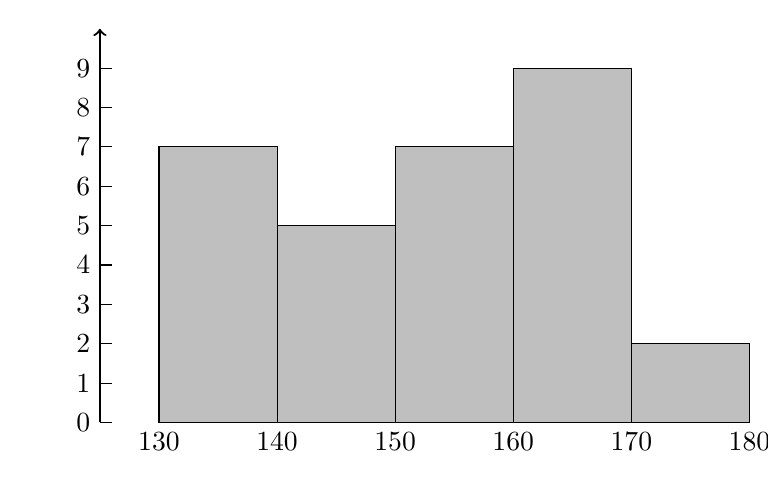
\begin{tikzpicture}[xscale=0.15,yscale=0.5]
      \draw[fill=lightgray] (130,0) rectangle (140,7);
      \draw[fill=lightgray] (140,0) rectangle (150,5);
      \draw[fill=lightgray] (150,0) rectangle (160,7);
      \draw[fill=lightgray] (160,0) rectangle (170,9);
      \draw[fill=lightgray] (170,0) rectangle (180,2);
      % x labels
      \foreach \x in {130, 140, ..., 180} {
        \draw (\x,0) node[anchor=north] {$\x$};
      }
      % y axis
      \draw[thick,->] (125,0) -- (125,10);
      % y labels
      \foreach \y in {0, 1, ..., 9} {
        \draw (125,\y) node[anchor=east] {$\y$} -- (126,\y);
      }
    \end{tikzpicture}
  \end{center}

  The histogram makes it easy to see in which range most of the
  heights are located and provides an overview of the distribution of
  the values in the data set.

}
\end{wex}    

With grouped data our estimates of central tendency will change
because we lose some information when we place each value in a range.
If all we have to work with is the grouped data, we do not know the
measured values to the same accuracy as before. The best we can do is
to assume that values are grouped at the centre of each range.

\begin{example}
Looking back to the previous worked example, we started with this data
set of learners' heights.
\begin{align*}
  \{&132;\ 132;\ 132;\ 133;\ 138;\ 139;\ 139;\ 140;\ 141;\ 142;\ 142;\ 146;\ 150;\ 150;\ 152;\\
    &152;\ 155;\ 156;\ 157;\ 160;\ 161;\ 162;\ 163;\ 164;\ 168;\ 168;\ 169;\ 169;\ 170;\ 172\}
\end{align*}
Note that the data are sorted here.

The mean of these data is $151,8$ and the median is $152$. The mode is
$132$, but remember that there are problems with computing the mode of
continuous quantitative data.

After grouping the data, we now have the data set shown below. Note
that each value is placed at the centre of its range and that the
number of times that each value is repeated corresponds exactly to the
counts in each range.
\begin{align*}
  \{&135;\ 135;\ 135;\ 135;\ 135;\ 135;\ 135;\ 145;\ 145;\ 145;\ 145;\ 145;\ 155;\ 155;\ 155;\\
    &155;\ 155;\ 155;\ 155;\ 165;\ 165;\ 165;\ 165;\ 165;\ 165;\ 165;\ 165;\ 165;\ 175;\ 175\}
\end{align*}
The grouping changes the measures of central tendency since each datum
is treated as if it occured at the centre of the range in which it was
placed.

The mean is now $153$, the median $155$ and the mode is $165$. This is
actually a better estimate of the mode, since the grouping showed in
which range the learners' heights were clustered.

\end{example}

\section{Dispersion}
The central tendency is not the only interesting or useful information
about a data set. The two data sets illustrated below have the same mean,
but are clearly quite different.

\begin{figure}[h]
  \begin{center}
    \begin{tabular}{cc}
      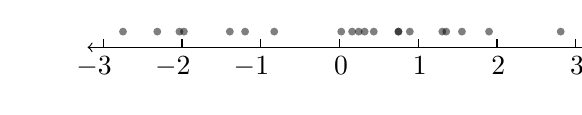
\begin{tikzpicture}
        \draw[<->] (-3.2, -0.2) -- (3.2, -0.2);
        \foreach \x in {-3, ..., 3} {
          \draw (\x, -0.2) -- (\x, -0.1);
          \draw (\x, -0.2) node[anchor=north east,xshift=0.23cm] {$\x$};
        }
        \foreach \x in {1.555, 1.899, 0.893, 0.160, 0.244, -0.829,
                        -1.199, -2.750, 0.022, -2.314, 2.809, 0.319,
                        -2.033, -1.976, 1.355, 0.749, 0.435, -1.393,
                        0.748, 1.306} {
          \fill[black,fill opacity=0.5] (\x,0) circle (0.05cm);
        }
      \end{tikzpicture}
      &
      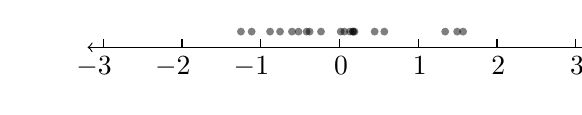
\begin{tikzpicture}
        \draw[<->] (-3.2, -0.2) -- (3.2, -0.2);
        \foreach \x in {-3, ..., 3} {
          \draw (\x, -0.2) -- (\x, -0.1);
          \draw (\x, -0.2) node[anchor=north east,xshift=0.23cm] {$\x$};
        }
        \foreach \x in {0.015, -0.418, 1.494, -0.882, 0.446, 0.061,
                        1.570, -0.755, 0.174, -0.604, -1.116, -0.380,
                        0.133, 0.569, -0.235, -0.521, 0.191, 0.169,
                        -1.252, 1.342} {
          \fill[black,fill opacity=0.5] (\x,0) circle (0.05cm);
        }
      \end{tikzpicture}
    \end{tabular}
  \end{center}
  \caption{Two sets of data with the same mean (0), but different spreads
    around the mean. Each circle represents one datum.}
\end{figure}

In this section we will look at measures of dispersion. Dispersion is
a general term for different statistics that describe how values or
distributed around the centre.

\subsection{Range}
\Definition{Range}{The range of a data set is the difference between
  the lowest value and the highest value in the set.}

The most straightforward of the dispersion measures is the range. The
range simply tells us how far apart the largest and smallest values in
a data set are. The range is very sensitive to outliers.

\begin{wex}{Range}{
    Find the range of the following data set.
    \begin{equation}
      \{1;\ 4;\ 5;\ 8;\ 6\; 7;\ 5;\ 6;\ 7;\ 4;\ 10;\ 9;\ 10\}
    \end{equation}
    What would happen if we removed the first datum from the set?
}{
  \westep{Find the minimum value.}

  The smallest value in the data set is $1$.

  \westep{Find the maximum value.}

  The largest value in the data set is $10$.

  \westep{Subtract the minimum value from the maximum value.}

  The range is $10-1=9$.

  \westep{Removing the first datum.}

  We don't usually do this, but if the first datum, $1$, were to be
  removed from the set, the minimum value would change from $1$ to
  $4$. This means that the range would change to $10-4=6$. This is
  very different from the previous value of the range.

  This is what we mean when we say that the range is sensitive to
  outliers. In the data set above, the value $1$ was not typical of
  the other values. It was an outlier and had a big influence on the
  range.

}
\end{wex}

We will look at a more general way of defining ranges later in this
section, but first we need to discuss the concept of percentiles.

\subsection{Percentiles}

\Definition{Percentile}{The $p$th percentile is the value, $v$, that
  divides a data set into two parts, such that $p$ per cent of the
  values in the data set are less than $v$ and $100-p$ per cent of the
  values are greater than $v$. Percentiles can lie in the range $0 \le
  p \le 100$.}

To understand percentiles properly, we need to distinguish between $3$
different aspects of a datum: its value, its rank and its
percentile. The value of a datum is what we measured and recorded
during an experiment or survey. The rank of a datum is its position in
the sorted data set. The percentile at which a particular datum is,
tells us what percentage of the values in the full data set are less
than this datum.

\begin{example}
  The table below summarises the value, rank and percentile of the
  data set
  \begin{equation}
    \{14,2;\ 13,9;\ 19,8;\ 10,3;\ 13,0;\ 11,1\}
  \end{equation}

  \begin{center}
    \begin{tabular}{ccc}
      \toprule
      value & rank & percentile \\
      \midrule
      $10,3$  & $1$    & 0 \\
      $11,1$  & $2$    & 20 \\
      $13,0$  & $3$    & 40 \\
      $13,9$  & $4$    & 60 \\
      $14,2$  & $5$    & 80 \\
      $19,8$  & $6$    & 100 \\
      \bottomrule
    \end{tabular}
  \end{center}

  Note that the rank describes the order of the data, from the
  smallest to the largest.

  As an example, $13,0$ is at the $40$th percentile since there are
  $2$ values less than $13,0$ and $3$ values greater than $13,0$.
  \begin{equation}
    \frac{2}{2+3} = 0,4 = 40\%
  \end{equation}
\end{example}

In general, the formula for finding the $p$th percentile in an ordered
data set with $n$ values is
\begin{equation}
  r = \frac{p}{100}\left(n-1\right)+1
\end{equation}
This gives us the rank, $r$, of the $p$th percentile. To find the
value of the $p$ percentile, we have to count from the first value in
the ordered data set up to the $r$th value.

Sometimes the rank will not be an integer. This means that the
percentile lies between two values in the data set. The convention is
to take the value halfway between the two values indicated by the
rank.

The figure below shows the relationship between rank and percentile
graphically. We have already encountered three percentiles in this
chapter: the median, the minimum and the maximum.

\begin{center}
  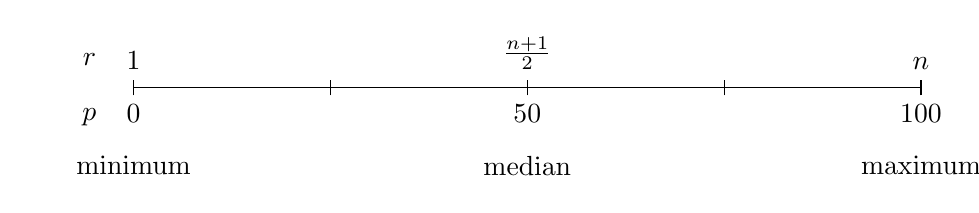
\begin{tikzpicture}[xscale=0.1]
    \draw (0,0) -- (100,0);
    \foreach \p in {0, 25, ..., 100} {
      \draw (\p, -0.1) -- (\p, 0.1);
    }
    \draw (0, -0.1) node[anchor=north east,xshift=-0.35cm,yshift=-0.05cm] {$p$};
    \draw (0, -0.1) node[anchor=north] {$0$};
    \draw (50, -0.1) node[anchor=north] {$50$};
    \draw (100, -0.1) node[anchor=north] {$100$};
    \draw (0, -0.75) node[anchor=north] {minimum};
    \draw (50, -0.75) node[anchor=north] {median};
    \draw (100, -0.75) node[anchor=north] {maximum};
    \draw (0, +0.1) node[anchor=south east,xshift=-0.35cm,yshift=+0.05cm] {$r$};
    \draw (0, +0.1) node[anchor=south] {$1$};
    \draw (50, +0.1) node[anchor=south] {$\frac{n+1}{2}$};
    \draw (100, +0.1) node[anchor=south] {$n$};
  \end{tikzpicture}
\end{center}

The median is defined as the value halfway in a sorted data set. Since
$50\% = \frac{1}{2}$, the median is exactly the same as the $50$th
percentile.  The minimum value is by definition the smallest and
therefore the leftmost value in a sorted set. This makes the minimum
equivalent to the $0$th percentile. Similarly, the maximum is
equivalent to the $100$th percentile.

\begin{wex}{Using the percentile formula}{
    Compute the minimum, maximum and median values of the following
    data set using the percentile formula.
    \begin{equation}
      \{14;\ 17;\ 45;\ 20;\ 19;\ 36;\ 7;\ 30;\ 8\}
    \end{equation}
}{
    \westep{Sort the values in the data set.}

    Before we can use the rank to find values in the data set, we
    always have to order the values from the smallest to the
    greatest. The sorted data set is
    \begin{equation}
      \{7;\ 8;\ 14;\ 17;\ 19;\ 20;\ 30;\ 36;\ 45\}
    \end{equation}

    \westep{Find the minimum.}

    We already know that the minimum value is the first value in the
    ordered data set. We will now confirm that the percentile formula
    gives the same answer. The minimum is equivalent to the $0$th
    percentile. According to the percentile formula the rank, $r$, of the
    $p = 0$th percentile in a data set with $n=9$ values is
    \begin{align}
      r &= \frac{p}{100}\left(n-1\right)+1 \\
        &= \frac{0}{100}\left(9-1\right)+1 \\
        &= 1
    \end{align}
    This confirms that the minimum value is the first value in the
    list, namely $7$.

    \westep{Find the maximum.}

    We already know that the maximum value is the last value in the
    ordered data set. The maximum is also equivalent to the $100$
    percentile. Using the percentile formula with $p=100$ and $n=9$,
    we find the rank of the maximum value as
    \begin{align}
      r &= \frac{p}{100}\left(n-1\right)+1 \\
        &= \frac{100}{100}\left(9-1\right)+1 \\
        &= 9
    \end{align}
    This confirms that the maximum value is the last (the $9$th) value
    in the list, namely $45$.

    \westep{Find the median.}

    The median is equivalent to the $50$th percentile. Using the
    percentile formula with $p=50$ and $n=9$, we find the rank of the
    median value as
    \begin{align}
      r &= \frac{50}{100}\left(n-1\right)+1 \\
        &= \frac{50}{100}\left(9-1\right)+1 \\
        &= \frac{1}{2}(8)+1 \\
        &= 5
    \end{align}
    This shows that the median is in the middle (at the $5$th position)
    of the ordered data set. Therefore the median value is $19$. 

}
\end{wex}

\Definition{Quartiles}{The quartiles are the three data values that
  divide an ordered data set into four groups, where each group
  contains an equal number of data values. The median ($50$th
  percentile) is the second quartile. The $25$th percentile can also
  be called the lower quartile, and the $75$th percentile the upper
  quartile.}

\begin{wex}{Quartiles}{
    Determine the quartiles of the following data set:
    \begin{equation}
      \{7;\ 45;\ 11;\ 3;\ 9;\ 35;\ 31;\ 7;\ 16;\ 40;\ 12;\ 6\}
    \end{equation}
}{
    \westep{Sort the data set.}
    \begin{equation}
      \{3;\ 6;\ 7;\ 7;\ 9;\ 11;\ 12;\ 16;\ 31;\ 35;\ 40;\ 45\}
    \end{equation}

    \westep{Find the ranks of the quartiles.}

    Using the percentile formula, we can find the rank of the $25$th,
    $50$th and $75$th percentiles as
    \begin{align}
      r_{25} &= \frac{25}{100}\left(12-1\right)+1 \\
            &= 3,75 \\
      r_{50} &= \frac{50}{100}\left(12-1\right)+1 \\
            &= 6,5 \\
      r_{75} &= \frac{75}{100}\left(12-1\right)+1 \\
            &= 9,25
    \end{align}

    \westep{Find the values of the quartiles.}

    Note that each of these ranks is a fraction, meaning that the
    value for each percentile is somewhere in between two values from
    the data set.

    For the $25$th percentile the rank is $3,75$, which is between
    the $3$rd and $4$th values. Since both these values are equal to
    $7$, the $25$th percentile is $7$.

    For the $50$th percentile (the median) the rank is $6,5$, meaning
    halfway between the $6$th and $7$th values. The $6$th value is
    $11$ and the $7$th value is $12$, which means that the median is
    $\frac{11+12}{2} = 11,5$.

    For the $75$th percentile the rank is $9,25$, meaning a quarter of
    the way from the $9$th value ($31$) to the $10$th value
    ($35$). Since there is a distance of $4$ between $31$ and $35$,
    the $75$th percentile is at $32$.

  }
\end{wex}

\subsection{Percentiles for grouped data}

In grouped data, the percentiles will lie somewhere inside a range,
rather than at a specific value. To find the range in which a
percentile lies, we still use the percentile formula to determine the
rank of the percentile and then find the range within which that rank
is.

\begin{wex}{Percentiles in grouped data}{
    The mathematics marks of $100$ grade $10$ learners at a school have
    been collected. The data are presented to you in the following
    table.
    \begin{center}
      \begin{tabular}{r@{\ }c@{\ }lc}
        \toprule
        \multicolumn{3}{c}{Percentage mark} & Number of learners \\
        \midrule
         $0$ & $ \le x < $ &  $20$ &  $2$ \\
        $20$ & $ \le x < $ &  $30$ &  $5$ \\
        $30$ & $ \le x < $ &  $40$ & $18$ \\
        $40$ & $ \le x < $ &  $50$ & $22$ \\
        $50$ & $ \le x < $ &  $60$ & $18$ \\
        $60$ & $ \le x < $ &  $70$ & $13$ \\
        $70$ & $ \le x < $ &  $80$ & $12$ \\
        $80$ & $ \le x < $ & $100$ & $10$ \\
        \bottomrule
      \end{tabular}
    \end{center}

    \begin{enumerate}
    \item Compute the mean of this grouped data set.
    \item In which interval is each of the quartiles of the data set?
    \item In which interval is the $30$th percentile of the data set?
    \end{enumerate}
}{

  \westep{Compute the mean.}

  Since we are given grouped data rather than the original ungrouped
  data, the best we can do is approximate the mean as if all the
  learners in each interval were located at the central value of the
  interval.

  \begin{equation}
    \frac{
         2 \cdot 10
      +  5 \cdot 25
      + 18 \cdot 35
      + 22 \cdot 45
      + 18 \cdot 55
      + 13 \cdot 65
      + 12 \cdot 75
      + 10 \cdot 90
    }{100}
    = 54\%
  \end{equation}

  \westep{Find the quartiles.}

  Since the data have been grouped, they have also already been
  sorted. Using the percentile formula and the fact that there are
  $100$ learners, we can find the rank of the $25$th, $50$th and
  $75$th percentiles as
  \begin{align}
    r_{25} &= \frac{25}{100}\left(100-1\right)+1 \\
          &= 24,75 \\
    r_{50} &= \frac{50}{100}\left(100-1\right)+1 \\
          &= 50,5 \\
    r_{75} &= \frac{75}{100}\left(100-1\right)+1 \\
          &= 75,25
  \end{align}

  Now we need to find in which ranges each of these ranks lie.
  \begin{itemize}
  \item For the first quartile, we have that there are $2 + 5 = 7$
    learners in the first two ranges combined and $2 + 5 + 18 = 25$
    learners in the first three ranges combined. This means that the
    first quartile (which has rank $r_{25} = 24,75$) lies somewhere in
    the range $30 \le x < 40$.
  \item For the second quartile (the median), we have that there are
    $2 + 5 + 18 + 22 = 47$ learners in the first four ranges combined
    and $47 + 18 = 65$ learners in the first five ranges
    combined. This means that the median (which has rank $r_{50} =
    50,5$) lies somewhere in the range $50 \le x < 60$.
  \item For the third quartile, we have that there are $65$ learners
    in the first five ranges combined and $65 + 13 = 78$ learners in
    the first six ranges combined. This means that the third quartile
    (which has rank $r_{75} = 75,25$) lies somewhere in the range $60
    \le x < 70$.
  \end{itemize}

  \westep{Find the $30$th percentile.}

  Using the same method as for the quartiles, we first find the rank
  of the $30$th percentile.
  \begin{align}
    r &= \frac{30}{100}\left(100-1\right)+1 \\
      &= 30,7
  \end{align}
  Now we have to find the range in which this rank lies. Since there
  are $25$ learners in the first $3$ ranges combined and $47$ learners
  in the first $4$ ranges combined, the $30$th percentile lies in the
  fourth range, namely $40 \le x < 50$.

}
\end{wex}

\subsection{Ranges}
The common ranges used are defined in terms of percentiles. The
overall range is simply the difference between the $100$th and the
$0$th percentile, that is between the maximum and minimum values in
the data set.

\Definition{Interquartile range}{The interquartile range is a
  measure of dispersion, which is calculated by subtracting the first
  quartile from the third quartile. This gives the range of the middle
  half of the data set.}

\Definition{Semi interquartile range}{The semi interquartile range is
  half of the interquartile range.}

\section{Combining different measures}
A common way of summarising the overall dataset is with the five
number summary and the box-and-whisker plot. These two represent
exactly the same information, numerically in the case of the five
number summary and graphically in the case of the box-and-whisker
plot.

The five number summary consists of the minimum value, the maximum
value and the three quartiles. Another way of saying this is that the
five number summary consists of the following percentiles: $0$th,
$25$th, $50$th, $75$th, $100$th.

The box-and-whisker plot shows these five percentiles, as in the figure
below. The box shows the interquartile range (the distance between the
first and third quartiles). A line inside the box shows the
median. The lines extending outside the box (the whiskers) show where
the minimum and maximum values lie.

\begin{center}
  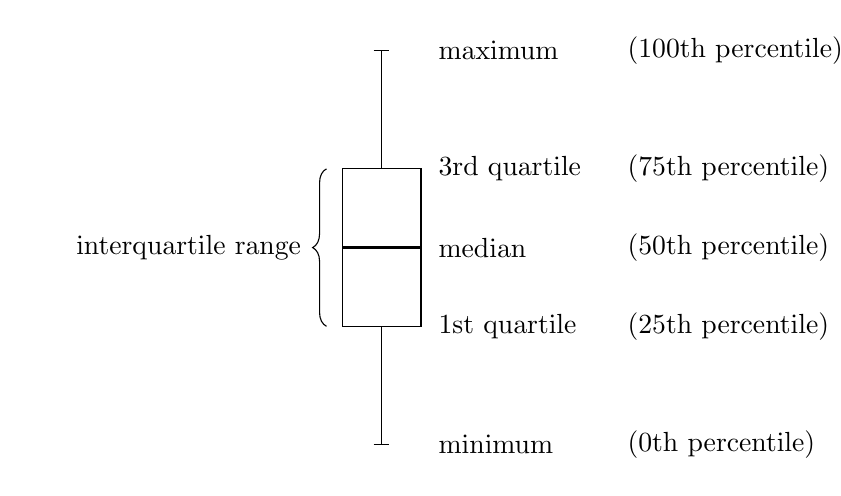
\begin{tikzpicture}
    \draw[thick] (-0.5, 0) -- (0.5, 0);
    \draw (-0.5, -1) rectangle (0.5, 1);
    \draw (0, -1) -- (0, -2.5);
    \draw (-0.1, -2.5) -- (0.1, -2.5);
    \draw (0, 1) -- (0, 2.5);
    \draw (-0.1, 2.5) -- (0.1, 2.5);
    \draw (0.6, 2.5) node[anchor=west] {maximum};
    \draw (0.6, 1) node[anchor=west] {$3$rd quartile};
    \draw (0.6, 0) node[anchor=west] {median};
    \draw (0.6, -1) node[anchor=west] {$1$st quartile};
    \draw (0.6, -2.5) node[anchor=west] {minimum};
    \draw (3, 2.5) node[anchor=west] {($100$th percentile)};
    \draw (3, 1) node[anchor=west] {($75$th percentile)};
    \draw (3, 0) node[anchor=west] {($50$th percentile)};
    \draw (3, -1) node[anchor=west] {($25$th percentile)};
    \draw (3, -2.5) node[anchor=west] {($0$th percentile)};
    \draw[decoration={brace,amplitude=0.5em},decorate] (-0.7,-1) -- (-0.7,1);
    \draw (-0.7,0) node[anchor=east,xshift=-0.2cm] {interquartile range};
  \end{tikzpicture}
\end{center}

\begin{wex}{Five number summary}{
    Draw a box and whisker diagram for the data set:
    \begin{equation}
      \{1,25;\ 1,5;\ 2,5;\ 2,5;\ 3,1;\ 3,2;\ 4,1;\ 4,25;\ 4,75;\ 4,8;\ 4,95;\ 5,1\}
    \end{equation}
}{
  \westep{Determine the minimum and maximum.}

  Since the data set is already sorted, we can read off the minimum as
  the first value, $1,25$, and the maximum as the last value, $5,1$.

  \westep{Determine the quartiles.}

  There are $12$ values in the data set. Using the percentile formula,
  we can determine that the median lies between the $6$th and $7$th
  values, making it
  \begin{equation}
    \frac{3,2 + 4,1}{2} = 3,65
  \end{equation}

  The first quartile lies between the $3$rd and $4$th values, making
  it
  \begin{equation}
    \frac{2,5 + 2,5}{2} = 2,5
  \end{equation}

  The third quartile lies between the $9$th and $10$th values, making
  it
  \begin{equation}
    \frac{4,75 + 4,8}{2} = 4,775
  \end{equation}

  This provides the five number summary of the data set and allows us
  to draw the box-and-whisker plot.

  \begin{center}
    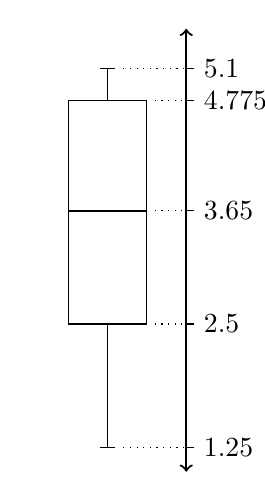
\begin{tikzpicture}[yscale=1.25]
      \def\median{3.65}
      \def\firstquartile{2.5}
      \def\thirdquartile{4.775}
      \def\minimum{1.25}
      \def\maximum{5.1}

      \draw (-0.5, \firstquartile) rectangle (0.5, \thirdquartile);
      \draw[thick] (-0.5, \median) -- (0.5, \median);
      \draw (0,    \firstquartile) -- (0,   \minimum);
      \draw (-0.1, \minimum) -- (0.1,       \minimum);
      \draw (0,    \thirdquartile) -- (0,   \maximum);
      \draw (-0.1, \maximum) -- (0.1,       \maximum);

      \draw[thick,<->] (1,1) -- (1,5.5);

      \foreach \y in {\minimum, \firstquartile, \median, \thirdquartile, \maximum} {
        \draw (1, \y) -- (1.1, \y) node[anchor=west] {$\y$};
      }
      \draw[dotted] (0.2, \maximum) -- (1, \maximum);
      \draw[dotted] (0.6, \thirdquartile) -- (1, \thirdquartile);
      \draw[dotted] (0.6, \median)  -- (1, \median);
      \draw[dotted] (0.6, \firstquartile) -- (1, \firstquartile);
      \draw[dotted] (0.2, \minimum) -- (1, \minimum);
    \end{tikzpicture}
  \end{center}
}
\end{wex}

\end{document}
